\newpage
\section{Bài toán 4: Ước lượng hệ số R}
\subsection{Cơ sở lý thuyết}
\subsubsection{Hệ số $R_0$}
Hệ số $R_0$ được gọi là Hệ số lây nhiễm cơ bản, cho biết rằng một ca nhiễm ban đầu có thể lây trực tiếp cho bao nhiêu người, và được tính bằng công thức:
\[R_0 = \frac{\beta}{\gamma}\]
Theo mô hình SIR được phát biểu ở (1), (2), (3), ta có được:
\[\frac{dR}{dt} + \frac{dI}{dt} = \frac{\beta}{N}IS\]
\[\frac{dR}{dt} = \gamma I\]
Từ đó, ta suy ra: 
\[R_0 = \frac{\beta}{\gamma} = \frac{N}{S}(1 + \frac{dI}{dR})\] \label{R0_I_R}
Do đó:
\[\frac{dI}{dR} = R_0 \frac{S}{N} - 1\]
Khi $R_0$ được ước lượng vào đầu mùa dịch, các khả năng sau có thể xảy ra:
\begin{itemize}
    \item $R_0 < 1$: Do $S \leq N$ nên $R_0 \frac{S}{N} - 1 < 0$. Mặt khác do các ca hồi phục được xem như đã miễn nhiễm thì $dR > 0$. Do đó $dI < 0$. Dịch bệnh không có khả năng bùng phát trong tương lai
    \item $R_0 > 1$: Trong khoảng thời gian đầu của mùa dịch, I và R không lớn, ta có thể xem $\frac{S}{N} \approx 1$, do đó $\frac{dI}{dR} = R_0 \frac{S}{N} - 1 > 0$. Tức là trong tương lai, số ca nhiễm bệnh vẫn còn tăng.
    Mặt khác, xét tại thời điểm ban đầu, ta có được:
    $$R_0 S(t = 0) > N$$
    Cùng với điều kiện $S \approx N$, có thể dự báo rằng trong tương lai, nếu $R_0$ không được kiểm soát, hầu như mọi người trong cộng đồng sẽ có thời điểm nào đó bị nhiễm bệnh, lúc đó ta nói rằng dịch bệnh bùng phát. $R_0$ càng lớn, tốc độ bùng phát dịch càng nhanh.
    \item $R_0 > 1$: $\frac{dI}{dR} \approx 0$. Dịch bệnh duy trì ổn định, không có khả năng bùng phát, nhưng chưa hoàn toàn được dập tắt.
\end{itemize}

\subsubsection{Ước lượng $R_0$}
    Với $R_0(\beta, \gamma) = \frac{\beta}{\gamma}$, $\pi(\beta, \gamma | X)$ là hàm phân bố xác suất của $(\beta, \gamma)$ khi có dữ liệu X. Giá trị trung bình của $R_0$ trên dữ liệu X là:
    $$E(R_0) = \int_{\beta, \gamma} \pi(\beta, \gamma | X)R_0(\beta, \gamma)d(\beta, \gamma)$$
    Công thức này không thể tính được trực tiếp, tuy nhiên ta có thể áp dụng công thức Bayes để đưa về:
    $$E(R_0) = \int_{\beta, \gamma} \frac{\pi(X | \beta, \gamma)\pi(\beta, \gamma)R_0(\beta, \gamma)}{\pi(X)}d(\beta, \gamma)$$
    Mặt khác, do $\pi(X)$ là dữ liệu đã được công bố chính thưc nên $\pi(X)$ là một hằng số và có thể được đưa ra ngoài dấu tích phân. Phần còn lại của tích phân sẽ tỉ lệ với $E(R_0)$.
    \begin{align}\label{approxR0}
        \begin{split}
            E(R_0) & \propto \int_{\beta, \gamma} \pi(X | \beta, \gamma)\pi(\beta, \gamma)R_0(\beta, \gamma)d(\beta, \gamma) \\
            & =E(\pi(X|\beta, \gamma)R_0(\beta, \gamma))\\
            & \approx \frac{1}{m} \Sigma_{i = 1}^{m} \pi(X|\beta_i, \gamma_i) \frac{\beta_i}{\gamma_i}
        \end{split}
    \end{align}
    $\beta$ và $\gamma$ được lấy mẫu từ phương pháp Metropolis-Hasting, là một thuật toán trong lớp Markov Chain Monte Carlo đã trình bày ở Bài toán 3.
    Ngoài ra, $\pi(X)$ có thể được tính bằng:
    \begin{align}
        \begin{split}
            \pi(X) & = \int_{\beta, \gamma} \pi(X | \beta, \gamma)\pi(\beta, \gamma)(\beta, \gamma) \\
            & \approx \frac{1}{m} \Sigma_{i = 1}^{m} \pi(X|\beta_i, \gamma_i)
        \end{split}
    \end{align}
    
    
\subsection{Code}
Nhóm sử dụng Matlab để hiện thực bài toán 4.Tuy $\pi(X)$ đã được giới thiệu một cách tính trong phần trên, nhưng việc tính toán chính xác $\pi(X)$ đã thất bại khi $\pi(X)$ luôn cho kết quả bằng 0. Do đó nhóm chỉ đi tính công thức ở (\ref{approxR0}) theo từng tuần trong file Singapore.csv, bắt đầu từ June 3rd 2020, kéo dài trong đúng 19 tuần. 
Nhắc lại công thức (\ref{R0_I_R}), vì số lượng người nhiễm bệnh và hồi phục (I + R) là nhỏ so với N, ta xem $\frac{N}{S} \approx 1$. Do đó sự thay đổi của $R0$ sẽ phụ thuộc chủ yếu vào $\frac{dI}{dR}$, cụ thể khi $R_0$ tăng thì $\frac{dI}{dR}$ cũng tăng và ngược lại. Do $E(R_0)$ xem như tỉ lệ với giá trị của biểu thức cuối cùng ở công thức (\ref{approxR0}) (gọi là K), ta sẽ đi tính K. Vì 0 < K < 1 và K rất gần với 0 nên để dễ quan sát, ta sẽ đi quan sát thông qua $log(K)$, cụ thể là $\frac{1}{|log(K)|}$ \\
\lstinputlisting{Code/baitoan3/R0_i.m}


\subsection{Kết quả}
    Nhập lệnh sau vào Command Windows trong Matlab:
    \begin{mdframed}[hidealllines=true,backgroundcolor=magenta!10]
	\begin{alltt}
	\textit{
	    >> R0_i('Singapore.csv',10000)
	}
	\end{alltt}
	\end{mdframed}
	
    \begin{figure}[h!]
	\begin{center}
		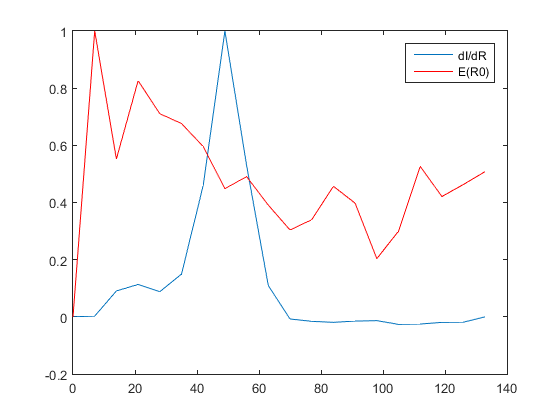
\includegraphics[scale=0.5]{Images/baitoan4/I-R-R0.png}
		\end{center}
		\caption{Đồ thị biểu diễn sự tương quan giữa $E(R_0)$ và $\frac{dI}{dR}$
	\end{figure}
